\section{图结构的谱刻画}
\label{sec:adjacency-spectral-structure}

如果只知道一张简单无向图$\mathcal G=(V,E)$的邻接谱$\lambda_1\ge\lambda_2\ge\cdots\ge\lambda_n$，我们能从中恢复出哪些图的结构参数，又能对哪些组合不变量给出上下界？

本节从局部到全局依次展开：第~\ref{sec:adjacency-low-spectral-moments}小节由二阶、三阶谱矩计数边和三角形，并结合顶点度从四阶谱矩计算四环数；第~\ref{sec:adjacency-diameter-bound}小节利用矩阵幂的线性无关性证明不同特征值的个数至少比图的直径多$1$；第~\ref{sec:adjacency-chromatic-bounds}小节结合导出子图的谱交错性质与单位根相位消去法，给出图色数$\chi(\mathcal G)$的谱上下界；第~\ref{sec:adjacency-hoffman-independence}小节通过中心化指示向量的Rayleigh商导出正则图最大独立集$\alpha(\mathcal G)$的Hoffman上界；最后，第~\ref{sec:adjacency-spectral-information}小节通过同谱非同构图反例，总结完整邻接谱的信息边界。

\subsection{局部结构}
\label{sec:adjacency-low-spectral-moments}

设简单无向图$\mathcal G=(V,E)$有$n=|V|$个顶点、$m=|E|$条边，顶点$v$的度记为$d_v$。由第~\ref{sec:adjacency-walk-counts}节的谱矩公式~\eqref{eq:adjacency-spectral-moments}，第$k$阶谱矩$\sum_{i=1}^n\lambda_i^k=\operatorname{tr}(\bm A^k)$等于全图长度为$k$的闭行走总数。当$k=1$时，简单无向图没有自环，一步闭行走条数为零，故一阶谱矩恒为$\operatorname{tr}(\bm A)=\sum_{i=1}^n\lambda_i=0$。下面依次分析$k=2,3,4$时的闭行走与局部子图计数。

\paragraph{边数}

考察长度为$2$的闭行走$u\to z\to u$。由于步数只有两步，第一步从起点$u$走到某个邻居$z$，第二步必须沿同一条边$\{u,z\}$原路退回$u$。因此，对顶点$u$的每一个邻居$z$，都恰好有一条两步闭行走$u\to z\to u$，从而对角元$(\bm A^2)_{u,u}=d_u$就是顶点$u$的度。

如图~\ref{fig:adjacency-edge-triangle-walks}(a)(b)所示，图中的每一条无向边$\{u,v\}\in E$恰好对应两条起点不同的两步闭行走：$u\to v\to u$（计入$(\bm A^2)_{u,u}$）和$v\to u\to v$（计入$(\bm A^2)_{v,v}$）。全图共有$m$条边，故两步闭行走总数为$2m$：
\[
\operatorname{tr}(\bm A^2)=\sum_{u\in V}d_u=\sum_{i=1}^n\lambda_i^2=2m.
\]

\paragraph{三角形数}

考察长度为$3$的闭行走$u\to v\to w\to u$。因为简单图没有自环，相邻两步的顶点必定互不相同（$v\neq u$，$w\neq v$，$u\neq w$），所以途中经过的三个顶点$u,v,w$必然两两互异，且两两之间都有边相连——它们在图中恰好围成一个三角形（三元环$C_3$）。

每一个三角形$\{u,v,w\}$会贡献多少条三步闭行走？如图~\ref{fig:adjacency-edge-triangle-walks}(c)(d)所示，固定一个起点$u$后，可以按$u\to v\to w\to u$和$u\to w\to v\to u$两个相反方向绕行，给出$2$条三步闭行走；三角形共有$3$个顶点可作为起点，每个起点各有$2$个绕行方向，因此每一个三角形恰好产生$3\times 2=6$条三步闭行走。

\begin{BookInlineFigure}
  \centering
  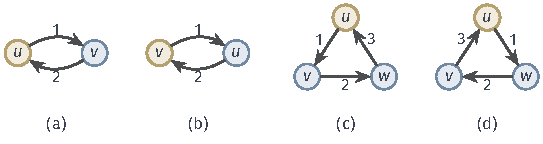
\includegraphics{figures/03-graphs/05-matrices-and-spectra/tikz/adjacency-edge-triangle-walks/figure.pdf}
  \caption{简单图上的两步与三步闭行走计数。浅黄色顶点标出闭行走的起点，箭头旁数字为步序。(a)(b) 同一条无向边$\{u,v\}$分别以$u$和$v$为起点各产生一条两步往返闭行走，共$2$条。(c)(d) 同一个三角形$\{u,v,w\}$在固定起点$u$下有顺、逆两个绕行方向；换遍三个起点共产生$3\times 2=6$条三步闭行走。}
  \label{fig:adjacency-edge-triangle-walks}
\end{BookInlineFigure}

记$t_3$为图$\mathcal G$中三角形（无序三元子集）的个数，则全图三步闭行走总数为$6t_3$。由此，图的边数$m$与三角形个数$t_3$可完全由二阶与三阶谱矩直接算出：
\begin{equation}
m=\frac12\operatorname{tr}(\bm A^2)=\frac12\sum_{i=1}^n\lambda_i^2,
\qquad
t_3=\frac16\operatorname{tr}(\bm A^3)=\frac16\sum_{i=1}^n\lambda_i^3.
\label{eq:adjacency-edge-triangle-counts}
\end{equation}

我们在四点环加对角边$\{1,3\}$的图上核对式~\eqref{eq:adjacency-edge-triangle-counts}。该图有$n=4$个顶点、$m=5$条边和$t_3=2$个三角形（即$\{1,2,3\}$与$\{1,3,4\}$）。其邻接矩阵$\bm A$与平方$\bm A^2$分别为
\[
\bm A=
\begin{bmatrix}
0&1&1&1\\
1&0&1&0\\
1&1&0&1\\
1&0&1&0
\end{bmatrix},
\qquad
\bm A^2=
\begin{bmatrix}
3&1&2&1\\
1&2&1&2\\
2&1&3&1\\
1&2&1&2
\end{bmatrix}.
\]
读取$\bm A^2$的四个对角元$(3,2,3,2)$，恰好是四个顶点的度$(d_1,d_2,d_3,d_4)$，二阶迹为$\operatorname{tr}(\bm A^2)=3+2+3+2=10$，除以$2$得边数$m=10/2=5$。再算$\bm A^3=\bm A^2\bm A$的对角元：例如$(\bm A^3)_{1,1}$是$\bm A^2$的第一行$(3,1,2,1)$与$\bm A$的第一列$(0,1,1,1)^\top$的内积，等于$1+2+1=4$（对应经过顶点$1$的两个三角形各贡献$2$个绕行方向）；同理可得$\bm A^3$的四个对角元为$(4,2,4,2)$，三阶迹为$\operatorname{tr}(\bm A^3)=4+2+4+2=12$，除以$6$得三角形数$t_3=12/6=2$。

\paragraph{四环数}

到了$k=4$步闭行走$v_0\to v_1\to v_2\to v_3\to v_0$，由于闭行走既可以沿简单四元环绕行，也可以在单条边或相邻两条边上来回折返，四阶谱矩$\operatorname{tr}(\bm A^4)$不再只包含四元环。按一条四步闭行走途中实际访问的不同顶点个数，可以将其不重不漏地分为三类（图~\ref{fig:adjacency-four-step-walks}）：
\begin{enumerate}
\item \textbf{第一类（只经过$2$个不同顶点）}：如图~\ref{fig:adjacency-four-step-walks}(a)所示，四步始终在同一条边$\{u,v\}$上来回折返两次。每条边有$u\to v\to u\to v\to u$和$v\to u\to v\to u\to v$两条记录，全图$m$条边共贡献$2m$条闭行走。
\item \textbf{第二类（经过$3$个不同顶点）}：如图~\ref{fig:adjacency-four-step-walks}(b)所示，在四个步序位置$v_0,v_1,v_2,v_3$中，必有某一个中心顶点$v$出现了两次，另外两个顶点$a,b$各出现一次（因无自环，重复顶点$v$只能隔一步出现在$v_0,v_2$或$v_1,v_3$位置，且$a,b$均与中心点$v$相邻，构成长为$2$的星形分支$a\text{--}v\text{--}b$）。对固定的一对公共邻居$\{a,b\}\subseteq N(v)$，共有$4$条四步闭行走：从中心$v$出发的$v\to a\to v\to b\to v$和$v\to b\to v\to a\to v$（$2$条），从端点$a$出发的$a\to v\to b\to v\to a$（$1$条），以及从端点$b$出发的$b\to v\to a\to v\to b$（$1$条）。在每个顶点$v\in V$处，从其$d_v$个邻居中选出一对无序邻居$\{a,b\}$共有$\binom{d_v}{2}$种选法，因此第二类闭行走总数为$4\sum_{v\in V}\binom{d_v}{2}$。
\item \textbf{第三类（经过$4$个不同顶点）}：如图~\ref{fig:adjacency-four-step-walks}(c)所示，四个顶点互不重复，首尾相连围成一个简单四元环$C_4$。设图中四元环的个数为$t_4$，每个四元环有$4$个可选起点、每个起点有顺逆$2$个绕行方向，共贡献$8t_4$条闭行走。
\end{enumerate}

\begin{BookInlineFigure}
  \centering
  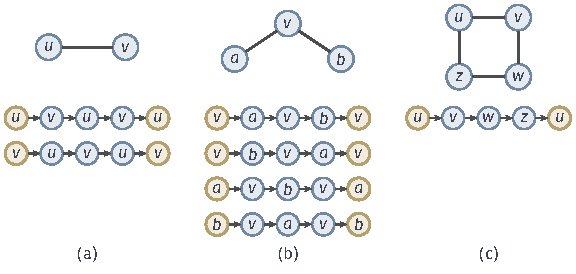
\includegraphics{figures/03-graphs/05-matrices-and-spectra/tikz/adjacency-four-step-walks/figure.pdf}
  \caption{按途中访问的不同顶点个数对四步闭行走分类。上排画出所使用的边，下排每一行从左到右列出一条五点访问序列，浅黄色标出重合的起点与终点。(a) 仅用$2$个顶点：在同一条边上来回折返两次（每条边$2$条）。(b) 使用$3$个顶点：在共享端点$v$的两条相邻边上各往返一次（每对相邻边$4$条）。(c) 使用$4$个不同顶点：沿简单四元环绕行一圈（每个四环$4\times 2=8$条）。}
  \label{fig:adjacency-four-step-walks}
\end{BookInlineFigure}

将三类闭行走条数相加，得到四阶谱矩分解公式：
\begin{equation}
\operatorname{tr}(\bm A^4)=\sum_{i=1}^n\lambda_i^4
=2m+4\sum_{v\in V}\binom{d_v}{2}+8t_4.
\label{eq:adjacency-four-cycle-count}
\end{equation}
在四点五边图上核对：第一类贡献$2m=10$；第二类中四个顶点的度依次为$3,2,3,2$，故$4\sum_v\binom{d_v}{2}=4\times(3+1+3+1)=32$；第三类中外圈$1\text{--}2\text{--}3\text{--}4\text{--}1$是唯一的四元环（$t_4=1$），贡献$8\times 1=8$；三项之和为$10+32+8=50$，与$\bm A^2$所有元素的平方和$\operatorname{tr}(\bm A^4)=\|\bm A^2\|_{\mathrm F}^2=(9+1+4+1)+(1+4+1+4)\times 2+(4+1+9+1)=50$完全一致。注意到式~\eqref{eq:adjacency-four-cycle-count}中出现了度平方和项$\sum_v\binom{d_v}{2}$：由于仅凭邻接谱一般无法唯一确定非正则图的度序列，从四阶谱矩$\operatorname{tr}(\bm A^4)$并不能单独反解出四元环个数$t_4$（第~\ref{sec:adjacency-cospectral-graphs}小节将给出具体反例）。

\subsection{直径的谱界}
\label{sec:adjacency-diameter-bound}

低阶谱矩刻画的是局部短闭行走。现在我们从另一个角度利用行走计数定理~\ref{thm:adjacency-walk-count}：如果图中两个顶点$u,v$之间的最短路距离为$k$，那么走少于$k$步绝对到不了$v$，而走恰好$k$步至少有一条路线能到达$v$。这一定性观察可以将图的全局直径与邻接矩阵不同特征值的个数联系起来。

回忆连通图$\mathcal G$中两点$u,v$之间的距离$\operatorname{dist}(u,v)$是连接它们的最短路径所含的边数，而图的直径$D=\max_{u,v\in V}\operatorname{dist}(u,v)$是所有点对距离的最大值。

取一对距离达到直径$D$的顶点，并写出连接它们的一条长度为$D$的最短路径：
\[
u_0\to u_1\to u_2\to\cdots\to u_D.
\]
对任意$k\in\{1,\ldots,D\}$，路径前缀$u_0\to u_1\to\cdots\to u_k$必然也是从$u_0$到$u_k$的最短路径（若存在少于$k$步的更短路径连接$u_0$与$u_k$，接上后缀$u_k\to\cdots\to u_D$就会得到一条总长小于$D$的从$u_0$到$u_D$的路径，与$\operatorname{dist}(u_0,u_D)=D$矛盾）。因此，$\operatorname{dist}(u_0,u_k)=k$。翻译成邻接矩阵幂的元素，就是：
\begin{equation}
(\bm A^j)_{u_0,u_k}=0\quad(\forall\,0\leq j<k),
\qquad\text{且}\qquad
(\bm A^k)_{u_0,u_k}\geq 1>0.
\label{eq:adjacency-diameter-echelon-entries}
\end{equation}
式~\eqref{eq:adjacency-diameter-echelon-entries}表明，$\bm I,\bm A,\bm A^2,\ldots,\bm A^D$这$D+1$个矩阵在一系列点对$(u_0,u_k)$处呈现出严格的“阶梯状”非零结构，由此可立即导出不同特征值个数的下界。

\begin{theorem}[直径的谱界]
\label{thm:adjacency-diameter-bound}
设连通简单无向图$\mathcal G$的直径为$D$，其邻接矩阵$\bm A$共有$r$个互不相同的特征值（不计重数）。则
\begin{equation}
r\geq D+1,\qquad\text{即}\qquad D\leq r-1.
\label{eq:adjacency-diameter-bound}
\end{equation}
\end{theorem}

\begin{proof}
我们分两步证明：（1）在$n\times n$矩阵空间中，$D+1$个矩阵幂$\bm I,\bm A,\bm A^2,\ldots,\bm A^D$线性无关；（2）若$\bm A$只有$r$个不同特征值，则$\bm A^r$可由$\bm I,\bm A,\ldots,\bm A^{r-1}$线性表出。

\textbf{第一步（$\bm I,\bm A,\ldots,\bm A^D$线性无关）}：用反证法。假设存在不全为零的实系数$c_0,c_1,\ldots,c_D$使得
\[
c_0\bm I+c_1\bm A+c_2\bm A^2+\cdots+c_D\bm A^D=\bm 0.
\]
令$k=\max\{j\in\{0,1,\ldots,D\}:c_j\neq 0\}$为最后一个非零系数的幂次，则上式化为
\[
c_0\bm I+c_1\bm A+\cdots+c_k\bm A^k=\bm 0,\qquad c_k\neq 0.
\]
在上面选出的最短路径$u_0\to u_1\to\cdots\to u_D$上，读取该矩阵等式在位置$(u_0,u_k)$处的元素：由式~\eqref{eq:adjacency-diameter-echelon-entries}，当$0\leq j<k$时$(\bm A^j)_{u_0,u_k}=0$，所有低次项在该位置全为$0$；唯一留下的最高次项为$c_k(\bm A^k)_{u_0,u_k}$。于是
\[
0=\sum_{j=0}^k c_j(\bm A^j)_{u_0,u_k}=c_k(\bm A^k)_{u_0,u_k}.
\]
但$c_k\neq 0$且$(\bm A^k)_{u_0,u_k}\geq 1>0$，乘积不可能等于$0$，矛盾。这证明了$\bm I,\bm A,\ldots,\bm A^D$这$D+1$个矩阵必定线性无关。

\textbf{第二步（利用特征根构造零化多项式）}：设$\bm A$的$r$个互不相同的实特征值为$\eta_1,\eta_2,\ldots,\eta_r$。构造$r$次首一多项式
\[
p(t)=(t-\eta_1)(t-\eta_2)\cdots(t-\eta_r)=t^r+b_{r-1}t^{r-1}+\cdots+b_1 t+b_0.
\]
因为实对称矩阵$\bm A$有一组由特征向量构成的完整正交基$\bm u_1,\ldots,\bm u_n$，每个基向量$\bm u_i$对应的特征值$\lambda_i$必定等于某个$\eta_j$。将矩阵多项式$p(\bm A)$作用在$\bm u_i$上，因子$(\bm A-\eta_j\bm I)\bm u_i=\bm 0$使整项归零：$p(\bm A)\bm u_i=\bm 0$（$\forall i=1,\ldots,n$）。在一个基上全为零的矩阵必为零矩阵，故
\[
p(\bm A)=\bm A^r+b_{r-1}\bm A^{r-1}+\cdots+b_1\bm A+b_0\bm I=\bm 0.
\]
这说明$\bm I,\bm A,\ldots,\bm A^r$这$r+1$个矩阵线性相关。若$r\leq D$，则$\{\bm I,\bm A,\ldots,\bm A^r\}$是线性无关组$\{\bm I,\bm A,\ldots,\bm A^D\}$的子集，不可能线性相关——矛盾。因此必有$r\geq D+1$。
\end{proof}

验证两个极端例子：完全图$K_n$（$n\geq 2$）的直径为$D=1$，定理~\ref{thm:adjacency-diameter-bound}要求它至少有$r\geq 2$个不同特征值，而第~\ref{sec:adjacency-complete-spectra}小节算出$K_n$恰有$n-1$和$-1$两个不同特征值（$r=2$），不等式取等；路径$P_n$的两端点距离为$D=n-1$，定理要求至少有$r\geq n$个不同特征值，因此$P_n$的全部$n$个特征值必定两两互异（单根），这与定理~\ref{prop:adjacency-path-spectrum}算出的$2\cos\bigl(\frac{k\pi}{n+1}\bigr)$完全一致。

\subsection{色数的谱界}
\label{sec:adjacency-chromatic-bounds}

图的正常顶点着色（proper vertex coloring）要求给每个顶点涂上一种颜色，使得任意一条边的两个端点颜色不同；所需的最少颜色数称为图的\emph{色数}（chromatic number），记为$\chi(\mathcal G)$。下面我们证明，仅凭最大特征值$\lambda_1$与最小特征值$\lambda_n$，就可以从上下两侧同时夹逼色数$\chi(\mathcal G)$。

在证明色数上界之前，需要先知道从图$\mathcal G$中删去若干顶点（连同关联的边）得到导出子图$\mathcal G'$时，邻接特征值如何变化。从矩阵上看，删去若干顶点相当于从邻接矩阵$\bm A$中删去相同编号的行和列，留下的子图邻接矩阵$\bm A_0$正是$\bm A$的一个主子矩阵（principal submatrix）。例如从三点路径$P_3$（特征值为$\sqrt 2,0,-\sqrt 2$）中删去端点$3$，留下的导出子图是单边图$K_2$（特征值为$1,-1$）。如图~\ref{fig:adjacency-interlacing-path}所示，$K_2$的两个特征值$1$和$-1$分别分别落在$P_3$相邻特征值所夹的区间$[0,\sqrt 2]$与$[-\sqrt 2,0]$内。

\begin{BookInlineFigure}
  \centering
  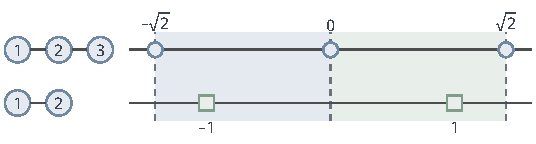
\includegraphics{figures/03-graphs/05-matrices-and-spectra/tikz/adjacency-interlacing-path/figure.pdf}
  \caption{删去三点路径$P_3$的端点$3$得到导出子图$K_2$时的特征值交错关系。上排圆点为$P_3$的邻接特征值$\sqrt2,0,-\sqrt2$，下排方点为二阶主子矩阵$K_2$的特征值$1,-1$，每个新特征值都落在相邻两个原特征值所夹的区间内。}
  \label{fig:adjacency-interlacing-path}
\end{BookInlineFigure}

这正是实对称矩阵的Cauchy交错定理（证明见\BookChapterRef{chap:condition-and-spectral-perturbation}{卷二"条件数与谱扰动"章}）：若$n$阶实对称矩阵$\bm A$的特征值为$\lambda_1\geq\cdots\geq\lambda_n$，其$k$阶主子矩阵$\bm A_0$的特征值为$\mu_1\geq\cdots\geq\mu_k$，则对每个$i=1,\ldots,k$都有$\lambda_i\geq\mu_i\geq\lambda_{i+n-k}$。特别地，取$i=1$可知：任意导出子图$\mathcal G'$的最大邻接特征值都不超过原图的最大邻接特征值，即$\lambda_1(\mathcal G')\leq\lambda_1(\mathcal G)$。需要注意，删顶点得到的是主子矩阵，可直接应用Cauchy交错定理；而单纯删边不删顶点只改变部分非对角元，并非主子矩阵截取。

有了导出子图的最大特征值界，下面同时证明色数$\chi(\mathcal G)$的Wilf上界与Hoffman下界。

\begin{theorem}[色数的谱上下界]
\label{thm:adjacency-chromatic-bounds}
设有限简单无向图$\mathcal G$至少含有一条边，色数为$\chi(\mathcal G)$，其最大与最小邻接特征值分别为$\lambda_1$与$\lambda_n$。则
\begin{equation}
1-\frac{\lambda_1}{\lambda_n}
\leq\chi(\mathcal G)
\leq 1+\lfloor\lambda_1\rfloor.
\label{eq:adjacency-chromatic-bounds}
\end{equation}
\end{theorem}

\begin{proof}
我们先证右侧上界$\chi(\mathcal G)\leq 1+\lfloor\lambda_1\rfloor$（Wilf界），再证左侧下界$\chi(\mathcal G)\geq 1-\lambda_1/\lambda_n$（Hoffman色数界）。

\textbf{第一步（上界证明：导出子图最小度与逆序贪心着色）}：任取原图$\mathcal G$的一个非空导出子图$\mathcal G'$，记其最小顶点度为$\delta(\mathcal G')$，平均度为$\overline d(\mathcal G')$。因为一组数的最小值不超过其平均值，且由定理~\ref{prop:adjacency-degree-bounds}（度下界）与主子矩阵Cauchy交错性质，有不等式链：
\[
\delta(\mathcal G')
\leq\overline d(\mathcal G')
\leq\lambda_1(\mathcal G')
\leq\lambda_1(\mathcal G)=\lambda_1.
\]
由于顶点度是整数，这保证了在$\mathcal G$的任意非空导出子图$\mathcal G'$中，总存在至少一个度不超过$\lfloor\lambda_1\rfloor$的顶点。

据此构造顶点删除序列：在原图$\mathcal G=\mathcal G_n$中选一个度$\leq\lfloor\lambda_1\rfloor$的顶点记为$v_n$并将其删去，得到$n-1$个顶点的导出子图$\mathcal G_{n-1}$；在$\mathcal G_{n-1}$中再选一个在$\mathcal G_{n-1}$内度$\leq\lfloor\lambda_1\rfloor$的顶点记为$v_{n-1}$并删去……如此继续，直到剩下一个顶点$v_1$。现在准备$\lfloor\lambda_1\rfloor+1$种颜色，按相反次序$v_1,v_2,\ldots,v_n$逐个将顶点放回并贪心着色：当放回顶点$v_j$时，它在已放回子图$\mathcal G_j=\{v_1,\ldots,v_j\}$中的邻居个数至多为$\lfloor\lambda_1\rfloor$，这些已着色的邻居至多占用了$\lfloor\lambda_1\rfloor$种颜色，因此在$\lfloor\lambda_1\rfloor+1$种颜色中必有至少一种空闲颜色可供$v_j$使用。故$\chi(\mathcal G)\leq 1+\lfloor\lambda_1\rfloor$。

\textbf{第二步（下界证明：单位根相位消去法）}：由于图至少有一条边，有$\lambda_1>0$；又因$\sum_{i=1}^n\lambda_i=\operatorname{tr}(\bm A)=0$，最小特征值必满足$\lambda_n<0$。

设图$\mathcal G$可以用$k=\chi(\mathcal G)$种颜色正常着色，将颜色编号为$c(u)\in\{0,1,\ldots,k-1\}$（$u\in V$），每条边$\{u,v\}\in E$的两端颜色不同：$c(u)\neq c(v)$。取$k$次本原单位根$\omega=\exp(2\pi\mathrm i/k)$，构造$n\times n$酉对角矩阵
\[
\begin{aligned}
\bm U&=\operatorname{diag}\bigl(\omega^{c(1)},\omega^{c(2)},\ldots,\omega^{c(n)}\bigr),\\
\bm U^*&=\bm U^{-1}=\operatorname{diag}\bigl(\omega^{-c(1)},\omega^{-c(2)},\ldots,\omega^{-c(n)}\bigr).
\end{aligned}
\]
对每个整数$j\in\{0,1,\ldots,k-1\}$，考察共轭矩阵$\bm U^{-j}\bm A\bm U^j$在位置$(u,v)$处的元素：
\[
\bigl(\bm U^{-j}\bm A\bm U^j\bigr)_{u,v}
=a_{u,v}\,\omega^{j(c(v)-c(u))}.
\]
将$j$从$0$到$k-1$对这$k$个矩阵求和：若$\{u,v\}\notin E$，则$a_{u,v}=0$，求和自然为$0$；若$\{u,v\}\in E$，因正常着色要求两端异色，$c(v)-c(u)\not\equiv 0\pmod k$，故公比$\eta=\omega^{c(v)-c(u)}\neq 1$且满足$\eta^k=1$，由等比数列求和公式有
\[
\sum_{j=0}^{k-1}\eta^j=\frac{1-\eta^k}{1-\eta}=0.
\]
这意味着在所有位置$(u,v)$上，$k$个共轭矩阵之和全为零矩阵：
\begin{equation}
\sum_{j=0}^{k-1}\bm U^{-j}\bm A\bm U^j=\bm 0.
\label{eq:adjacency-chromatic-phase-cancellation}
\end{equation}

现在取$\bm A$属于最大特征值$\lambda_1$的实单位特征向量$\bm x\in\mathbb R^n$（$\|\bm x\|_2=1$，$\bm x^\top\bm A\bm x=\lambda_1$），用$\bm x^\top$和$\bm x$夹乘式~\eqref{eq:adjacency-chromatic-phase-cancellation}两端，并令$\bm z^{(j)}=\bm U^j\bm x\in\mathbb C^n$：
\[
0=\sum_{j=0}^{k-1}\bm x^\top\bigl(\bm U^{-j}\bm A\bm U^j\bigr)\bm x
=\bm x^\top\bm A\bm x+\sum_{j=1}^{k-1}(\bm z^{(j)})^*\bm A\bm z^{(j)}.
\]
由于$\bm U^j$的对角元模长全为$1$，每个$\bm z^{(j)}=\bm U^j\bm x$仍是单位向量（$(\bm z^{(j)})^*\bm z^{(j)}=\|\bm x\|_2^2=1$）。在实对称矩阵$\bm A$的正交特征基下展开，任意复单位向量的二次型$(\bm z^{(j)})^*\bm A\bm z^{(j)}$都是特征值$\lambda_1,\ldots,\lambda_n$的凸组合，故不小于最小特征值$\lambda_n$。将$j=0$项的$\lambda_1$与其余$k-1$项的下界$\lambda_n$代入上式：
\[
0\geq\lambda_1+(k-1)\lambda_n.
\]
将负项$-(k-1)\lambda_n$移到左端并同除以$-\lambda_n>0$（注意$\lambda_n<0$），得$k-1\geq\frac{\lambda_1}{-\lambda_n}$，即$k\geq 1-\frac{\lambda_1}{\lambda_n}$。
\end{proof}

我们在完全图$K_n$和五元环$C_5$上检验定理~\ref{thm:adjacency-chromatic-bounds}。对完全图$K_n$，$\lambda_1=n-1,\lambda_n=-1$，下界给出$1-\frac{n-1}{-1}=n$，上界给出$1+\lfloor n-1\rfloor=n$，上下界同时取等，唯一确定$\chi(K_n)=n$。对五元奇环$C_5$，由定理~\ref{prop:adjacency-cycle-spectrum}知$\lambda_1=2$，$\lambda_5=2\cos(4\pi/5)=-\frac{1+\sqrt 5}{2}\approx -1.618$，下界给出
\[
\chi(C_5)\geq 1+\frac{2}{(1+\sqrt 5)/2}=1+\sqrt 5-1=\sqrt 5\approx 2.236.
\]
因为色数必须是整数，向上取整立得$\chi(C_5)\geq 3$；而上界给出$\chi(C_5)\leq 1+2=3$，上下界共同确定$\chi(C_5)=3$。

\subsection{独立数的谱界}
\label{sec:adjacency-hoffman-independence}

在图的正常着色中，涂同一种颜色的所有顶点彼此之间不能有边相连。这种两两互不相邻的顶点子集$S\subseteq V$称为图的\emph{独立集}（independent set），图所含最大独立集的顶点数称为\emph{独立数}（independence number），记为$\alpha(\mathcal G)$。显然，若用$\chi(\mathcal G)$种颜色把$n$个顶点分成$\chi(\mathcal G)$个独立集，每个独立集至多含$\alpha(\mathcal G)$个顶点，必有$n\leq\chi(\mathcal G)\alpha(\mathcal G)$，即$\chi(\mathcal G)\geq n/\alpha(\mathcal G)$。那么，能否直接用邻接谱给出独立数$\alpha(\mathcal G)$的上界？

如果直接取独立集$S$的$0$--$1$指示向量$\bm 1_S$（在$S$内取$1$、在$S$外取$0$），由于$S$内部没有任何边，二次型$\bm 1_S^\top\bm A\bm 1_S=0$恒等于零，从中读不出$|S|$的大小。为了把独立集向外部发出的边数信息引入二次型，同时也为了消去常向量$\bm 1$方向（最大特征值$\lambda_1=d$方向）的分量，我们在$d$正则图上从指示向量$\bm 1_S$中减去它的全图平均值$s/n$（其中$s=|S|$），构造中心化测试向量
\[
\bm x=\bm 1_S-\frac{s}{n}\bm 1.
\]
经过中心化后，$\bm x$在$S$内的$s$个顶点上取正值$1-\frac{s}{n}$，在$S$外的$n-s$个顶点上取负值$-\frac{s}{n}$，且全部$n$个分量之和为零（$\bm 1^\top\bm x=0$，即$\bm x\perp\bm 1$）。此时从$S$连向$V\setminus S$的跨界边两端一正一负，产生负的二次型，正好受最小特征值$\lambda_n$的下方约束。

\begin{theorem}[独立数的Hoffman界]
\label{thm:adjacency-hoffman-independence}
设$\mathcal G$是$n$个顶点的简单$d$正则无向图（$d\geq 1$），最小邻接特征值为$\lambda_n$。则其独立数$\alpha(\mathcal G)$满足
\begin{equation}
\alpha(\mathcal G)\leq n\,\frac{-\lambda_n}{d-\lambda_n}.
\label{eq:adjacency-hoffman-independence}
\end{equation}
\end{theorem}

\begin{proof}
任取$\mathcal G$的一个非空独立集$S\subseteq V$，记$s=|S|\geq 1$。因为$d\geq 1$，图中每个顶点都有边相连，独立集不可能包含全部顶点，故$1\leq s<n$。令$\bm x=\bm 1_S-\frac{s}{n}\bm 1$，则$\bm 1^\top\bm x=s-\frac{s}{n}\cdot n=0$，即$\bm x\in\bm 1^\perp$。

我们分别计算向量$\bm x$的欧氏长度平方$\|\bm x\|_2^2$和二次型$\bm x^\top\bm A\bm x$。首先计算长度平方：因为$\bm 1_S^\top\bm 1_S=s$且$\bm 1_S^\top\bm 1=s$，展开得
\[
\begin{aligned}
\|\bm x\|_2^2
&=\Bigl(\bm 1_S-\frac{s}{n}\bm 1\Bigr)^\top\Bigl(\bm 1_S-\frac{s}{n}\bm 1\Bigr)
=s-2\frac{s}{n}\cdot s+\frac{s^2}{n^2}\cdot n\\
&=s-\frac{s^2}{n}
=s\Bigl(1-\frac{s}{n}\Bigr)>0.
\end{aligned}
\]

再计算二次型$\bm x^\top\bm A\bm x$：利用双线性展开，
\[
\bm x^\top\bm A\bm x
=\bm 1_S^\top\bm A\bm 1_S
-2\frac{s}{n}\bm 1_S^\top\bm A\bm 1
+\frac{s^2}{n^2}\bm 1^\top\bm A\bm 1.
\]
逐项化简右端三项：第一项$\bm 1_S^\top\bm A\bm 1_S=\sum_{u,v\in S}a_{u,v}$等于独立集$S$内部边数的两倍，由于$S$是独立集、内部无边，故$\bm 1_S^\top\bm A\bm 1_S=0$；第二项利用$d$正则图的性质$\bm A\bm 1=d\bm 1$，得$\bm 1_S^\top\bm A\bm 1=d(\bm 1_S^\top\bm 1)=ds$；第三项同样由$\bm A\bm 1=d\bm 1$，得$\bm 1^\top\bm A\bm 1=d(\bm 1^\top\bm 1)=dn$。将三项结果代回，得到
\[
\bm x^\top\bm A\bm x
=0-2\frac{s}{n}(ds)+\frac{s^2}{n^2}(dn)
=-\frac{ds^2}{n}.
\]

现在应用Rayleigh商的最小特征值下界：对任意非零向量$\bm x$，都有$\bm x^\top\bm A\bm x\geq\lambda_n\|\bm x\|_2^2$。将上面算出的$\bm x^\top\bm A\bm x$与$\|\bm x\|_2^2$代入：
\[
-\frac{ds^2}{n}\geq\lambda_n\Bigl(s-\frac{s^2}{n}\Bigr).
\]
在不等式两端同除以正数$s>0$，得
\[
-\frac{ds}{n}\geq\lambda_n-\lambda_n\frac{s}{n}
\quad\Longrightarrow\quad
(d-\lambda_n)\frac{s}{n}\leq -\lambda_n.
\]
因为$d\geq 1$且$\lambda_n<0$，必有$d-\lambda_n>0$。两端同除以$d-\lambda_n$再乘以$n$，即得$s\leq n\frac{-\lambda_n}{d-\lambda_n}$。对最大独立集取$s=\alpha(\mathcal G)$，式~\eqref{eq:adjacency-hoffman-independence}得证。
\end{proof}

从证明过程还可以看到：在$d$正则图上，将式~\eqref{eq:adjacency-hoffman-independence}代入色数与独立数的关系$\chi(\mathcal G)\geq\frac{n}{\alpha(\mathcal G)}$，立得$\chi(\mathcal G)\geq\frac{d-\lambda_n}{-\lambda_n}=1-\frac{d}{\lambda_n}=1-\frac{\lambda_1}{\lambda_n}$，这从独立集视角再次印证了定理~\ref{thm:adjacency-chromatic-bounds}中的Hoffman色数下界。

检验两个例子：对偶数长环$C_{2r}$（$d=2,\lambda_n=-2$）或等侧完全二部图$K_{r,r}$（$d=r,\lambda_n=-r$），Hoffman界给出$\alpha(\mathcal G)\leq n\frac{d}{2d}=\frac{n}{2}$，取二部划分的任一侧即达到等号；对五元环$C_5$（$n=5,d=2,\lambda_5=-\frac{1+\sqrt 5}{2}$），Hoffman界给出$\alpha(C_5)\leq 5\cdot\frac{(1+\sqrt 5)/2}{2+(1+\sqrt 5)/2}=\sqrt 5\approx 2.236$，由于独立数是整数，向下取整得$\alpha(C_5)\leq 2$，任取两个不相邻顶点即达到最大值$2$。

\subsection{同谱图}
\label{sec:adjacency-spectral-information}
\label{sec:adjacency-cospectral-graphs}

综合前面几节的结果，我们可以对“完整邻接谱究竟能告诉我们多少图结构信息”作一全面梳理。

\paragraph{邻接谱确定的图不变量}

给定简单无向图$\mathcal G$的全部$n$个邻接特征值$\lambda_1\ge\cdots\ge\lambda_n$，以下不变量与界可由谱确定（界不等于相应参数的精确值）：
\begin{enumerate}
\item \textbf{顶点数$n$、边数$m$与三角形个数$t_3$}：特征值总个数就是顶点数$n$；由式~\eqref{eq:adjacency-edge-triangle-counts}，$m=\frac12\sum_{i=1}^n\lambda_i^2$，三角形个数$t_3=\frac16\sum_{i=1}^n\lambda_i^3$，以及任意阶$k$步闭行走的总数$\sum_{i=1}^n\lambda_i^k$。
\item \textbf{是否为正则图}：由定理~\ref{prop:adjacency-degree-bounds}，先由二阶谱矩算出平均度$\overline d=\frac1n\sum_{i=1}^n\lambda_i^2$，再检查最大特征值是否满足$\lambda_1=\overline d$。因为常向量$\bm 1$达到最大Rayleigh商$\lambda_1$当且仅当$\bm A\bm 1=\lambda_1\bm 1$（无论图是否连通），所以$\mathcal G$是正则图当且仅当$\lambda_1=\frac1n\sum_{i=1}^n\lambda_i^2$。
\item \textbf{是否为二部图}：由定理~\ref{thm:adjacency-bipartite-spectral-symmetry}的第1条，$\mathcal G$是二部图当且仅当全部特征值关于原点对称（$\lambda_i=-\lambda_{n+1-i},\forall i$）。
\item \textbf{直径、色数与独立数的硬性范围约束}：不同特征值个数给出连通图直径上界$D\leq r-1$，最大与最小特征值给出色数范围$1-\lambda_1/\lambda_n\leq\chi(\mathcal G)\leq 1+\lfloor\lambda_1\rfloor$及正则图独立数上界$\alpha(\mathcal G)\leq n\frac{-\lambda_n}{d-\lambda_n}$。
\end{enumerate}

\paragraph{同谱非同构图}

尽管邻接谱包含丰富的代数信息，但它不能唯一确定图的同构类。如果两张图$\mathcal G$与$\mathcal H$的邻接谱（作为带重数的多重集）完全相同，则称它们为\term{同谱图}（cospectral graphs，或等谱图）。两张同构的图仅相差顶点重新编号（即邻接矩阵相差置换相似变换$\bm P\bm A\bm P^\top$），因此必然同谱；但反过来，存在大量结构截然不同、却拥有完全相同邻接谱的非同构图。

最经典的一对五顶点同谱非同构图如图~\ref{fig:adjacency-cospectral-pair}所示：左图是星图$K_{1,4}$，右图是四元环与一个孤立顶点的不交并$C_4\sqcup K_1$。

\begin{figure}[!htb]
  \centering
  \begingroup
\definecolor{GraphSpectrumNode}{HTML}{E5EAF0}
\definecolor{GraphSpectrumOutline}{HTML}{7188A3}
\definecolor{GraphSpectrumEdge}{HTML}{4C4D4F}
\definecolor{GraphSpectrumText}{HTML}{3B4252}
\begin{tikzpicture}[x=8mm,y=8mm,
  vertex/.style={circle,inner sep=0pt,minimum size=2.7mm,
    fill=GraphSpectrumNode,draw=GraphSpectrumOutline,line width=.65pt},
  every path/.style={line width=.8pt},
  title/.style={text=GraphSpectrumText,font=\footnotesize}]
  \begin{scope}
    \node[vertex] (s) at (0,0) {};
    \node[vertex] (l1) at (-.8,.8) {};
    \node[vertex] (l2) at (.8,.8) {};
    \node[vertex] (l3) at (.8,-.8) {};
    \node[vertex] (l4) at (-.8,-.8) {};
    \foreach \v in {l1,l2,l3,l4} {
      \draw[GraphSpectrumEdge] (s) -- (\v);
    }
    \node[title] at (0,-1.3) {$K_{1,4}$};
  \end{scope}
  \begin{scope}[xshift=29mm]
    \node[vertex] (c1) at (-.8,.8) {};
    \node[vertex] (c2) at (.8,.8) {};
    \node[vertex] (c3) at (.8,-.8) {};
    \node[vertex] (c4) at (-.8,-.8) {};
    \node[vertex] at (1.6,0) {};
    \draw[GraphSpectrumEdge] (c1) -- (c2) -- (c3) -- (c4) -- (c1);
    \node[title] at (.3,-1.3) {$C_4\sqcup K_1$};
  \end{scope}
\end{tikzpicture}
\endgroup

  \caption{最小的一对简单无向邻接同谱非同构图。(a) 左图星图$K_{1,4}$由$1$个中心顶点连接$4$个叶子顶点，连通且无环。(b) 右图$C_4\sqcup K_1$由一个四元环与一个孤立顶点组成，不连通且含四元环。两图的邻接谱同为$\{2,0,0,0,-2\}$。}
  \label{fig:adjacency-cospectral-pair}
\end{figure}

利用第~\ref{sec:adjacency-standard-spectra}节的结果立即可以核对两图的谱：左图$K_{1,4}$是$p=1,q=4$的完全二部图，由定理~\ref{prop:adjacency-bipartite-complete-spectrum}，其非零特征值为$\pm\sqrt{1\times 4}=\pm 2$，零特征值重数为$1+4-2=3$，故谱为$\{2,0,0,0,-2\}$；右图$C_4\sqcup K_1$是分块对角矩阵，$C_4$的特征值为$2,0,0,-2$，孤立顶点$K_1$添入一个特征值$0$，合起来的谱也是$\{2,0,0,0,-2\}$。

两张图的全部$5$个特征值一模一样，但它们展示出邻接谱丢失的三项重要结构信息：
\begin{enumerate}
\item \textbf{邻接谱不能判定连通性}：$K_{1,4}$是连通图（一棵树），而$C_4\sqcup K_1$不连通（有$2$个连通分量）。（第~\ref{chap:graph-laplacian-matrix}章将看到，拉普拉斯矩阵的零特征值重数恰等于连通分量个数，从而弥补邻接谱的这一缺陷。）
\item \textbf{邻接谱不能确定度序列}：$K_{1,4}$的度序列是$(4,1,1,1,1)$，而$C_4\sqcup K_1$的度序列是$(2,2,2,2,0)$。虽然两图的度之和都是$2m=8$，但各自的度分布完全不同。
\item \textbf{邻接谱不能确定四元环个数$t_4$}：$K_{1,4}$是树，四元环个数$t_4=0$；而$C_4\sqcup K_1$含有$t_4=1$个四元环。
\end{enumerate}

\paragraph{闭行走的补偿机制}

既然两图同谱，它们的任意阶谱矩$\operatorname{tr}(\bm A^k)=\sum_{i=1}^5\lambda_i^k$都相等，特别是四阶谱矩均为$\operatorname{tr}(\bm A^4)=2^4+(-2)^4=32$。为什么一张没有四元环（$t_4=0$）、另一张有一个四元环（$t_4=1$），四步闭行走的总数却同样是$32$？

用式~\eqref{eq:adjacency-four-cycle-count}把两图的四步闭行走按三类拆开：在星图$K_{1,4}$上，单边往返（第一类）有$2m=8$条，中心点度为$4$、有$\binom{4}{2}=6$对相邻边从而贡献$4\times 6=24$条星形分支往返（第二类），四元环绕行（第三类）为$8\times 0=0$条，合计$8+24+0=32$条。

而在$C_4\sqcup K_1$上，单边往返（第一类）也是$2m=8$条，四环上的$4$个顶点度均为$2$、各有$\binom{2}{2}=1$对相邻边从而只贡献$4\times(1+1+1+1)=16$条第二类行走，但多出的$1$个四元环恰好补上了$8\times 1=8$条第三类绕行，合计同样是$8+16+8=32$条。

可以看到，$K_{1,4}$靠度为$4$的中心节点多产生了$8$条三顶点折返行走，恰好与$C_4\sqcup K_1$沿四元环绕行产生的$8$条行走在求和后相抵。迹算子$\operatorname{tr}(\bm A^k)$只汇总闭行走的总条数，抹去了闭行走究竟来自星形高次度节点还是来自四元环的拓扑细节。

总结而言，邻接谱是图同构的一个必要非充分不变量：若两张图的邻接谱不同，立即可断定它们不同构；但若邻接谱相同，仅凭特征值还不足以确认同构。下一节我们将进一步考察：如果把原图的顶点按对称角色聚合成若干块，用更小的商矩阵代替原邻接矩阵，这种粗粒化的“商谱”又能保留多少谱信息？
